% !TeX root = ../pythonTutorial.tex
\chapter{Ein- und Ausgabe}
\label{chapter:inputoutput}

In Python gibt es verschiedene Methoden um Daten vom Benutzer entgegenzunehmen und Daten dem Benutzer zur Verf�gung zustellen.

% !TeX root = ../../pythonTutorial.tex
\section{Konsolenausgabe mit print()}
\label{printInOut}

Die \emph{print()}-Funktion hat vielerlei Nutzen und wird entsprechend oft verwendet. Daher ist es definitiv sinnvoll, sich mit ihr vertraut zu machen.

\begin{lstlisting}[language=Python, label=printInOut:lst:printDefault]
# die Print-Methode

print(value1, value2, ..., sep=" ", 
    end="\n", file=sys.stdout, flush= false))
\end{lstlisting}

In Listing (\ref{printInOut:lst:printDefault}) sind die Parameter von \emph{print()} zu sehen. Die auszugebenden Werte stehen an erster Stelle (value1, value2, ...), hierbei handelt es sich um eine beliebige Anzahl an Werten. Der Parameter \emph{sep} bildet den Seperator zwischen den Werten und hat als Standardwert das Leerzeichen.
\randnotiz{Seperator}
In Listing \ref{printInOut:lst:printSeperator} k�nnen wir sehen, dass wir durch Angabe eines Seperators eine bessere Lesbarkeit erreichen k�nnen.

\begin{lstlisting}[language=Python, label=printInOut:lst:printSeperator]
# die Print-Methode mit Seperator

print(1,2,3)
# Ausgabe: 1 2 3

print(1,2,3, sep=" | ")
# Ausgabe: 1 | 2 | 3
\end{lstlisting}

Nach dem Seperator folgt der \emph{end}-Parameter, dieser f�gt standardgem�� einen Zeilenumbruch (\textbackslash n) an das Ende der Ausgabe.
\randnotiz{End-Angabe}

\begin{lstlisting}[language=Python, label=printInOut:lst:printEnd]
# die Print-Methode mit End-Angabe

print("Satz mit Zeilenumbruch")
print("N�chster Satz")
# Ausgabe:
# Satz mit Zeilenumbruch
# N�chster Satz

print("Satz mit Punkt und Leerzeichen." , end=". ")
print("N�chster Satz)
# Ausgabe: 
# Satz mit Punkt und Leerzeichen. N�chster Satz
\end{lstlisting}

Der \emph{file}-Parameter bestimmt den Datenstrom (\emph{Stream}) f�r den Output. In \emph{sys.stdout} steht f�r die Konsole. 
\randnotiz{Output-Stream}
M�chten wir den Output bspw. in eine Textdatei schreiben, dann k�nnen wir diese als Ziel des Datenstroms festlegen.

\begin{lstlisting}[language=Python, label=printInOut:lst:printFile]
# die Print-Methode mit Ausgabe in Textdatei

# open() -> festlegen einer Textdatei als Stream
# "w" steht f�r 'write' und gibt an,
# dass wir etwas in die Datei schreiben m�chten

txtFile = open(beispielText.txt, "w")
print("Hello, World.", file="txtFile")
txtFile.close()
# close() schlie�t den Stream
\end{lstlisting}




% !TeX root = ../../pythonTutorial.tex
\section{Formatierung von Strings}
\label{formatInOut}

Es w�re sicherlich hilfreich, wenn wir die String-Ausgaben nach belieben formatieren k�nnten. Bisher haben wir den Seperator von \emph{print()} kennengelernt - dieser ist von seiner Funktionsweise jedoch stark beschr�nkt. Python bietet uns hierf�r die \emph{format()}-Methode an, vorher betrachten wir aber die Modulo-Arithmetik und machen uns mit den Formatierungszeichen vertraut.
 
Mittels Modulo-Arithmetik \randnotiz{Modulo-
Arithmetik} leiten wir ein Formatierungszeichen ein. Dieses gilt als Platzhalter f�r einen Wert.

\begin{lstlisting}[language=Python, label=formatInOut:lst:modulo]
# Modulo-Arithmetik

print("K�rper: %s , Fl�che: %f m" %
	('Dreieck', 42.6))
	
# Ausgabe:
# K�rper: Dreieck , Fl�che: 42.6
\end{lstlisting}

Bei "'K�rper"' setzen wir den ersten Platzhalter mit "'\%s"'. Die Reihenfolge der Platzhalter setzt fest, welcher Wert anschlie�end eingebunden wird. Der erste Platzhalter tr�gt also den ersten Wert, der nach dem Ausgabetext folgt, der zweite den zweiten und so weiter.

\warning{Die einzusetzenden Werte werden nach dem String mittels Modulo als Tupel festgelegt!}

Das Formatierungszeichen nach dem Modulo bestimmt den Datentyp des Wertes.
Bei "'s"' handelt es sich um einen String, bei "'f"' um ein \emph{float}.
In folgender Tabelle sind die m�glichen Formatierungszeichen aufgelistet.

\begin{figure}
	\caption{Formatierungszeichen und ihre Bedeutung \cite{pythonFormat}}
	\centering
	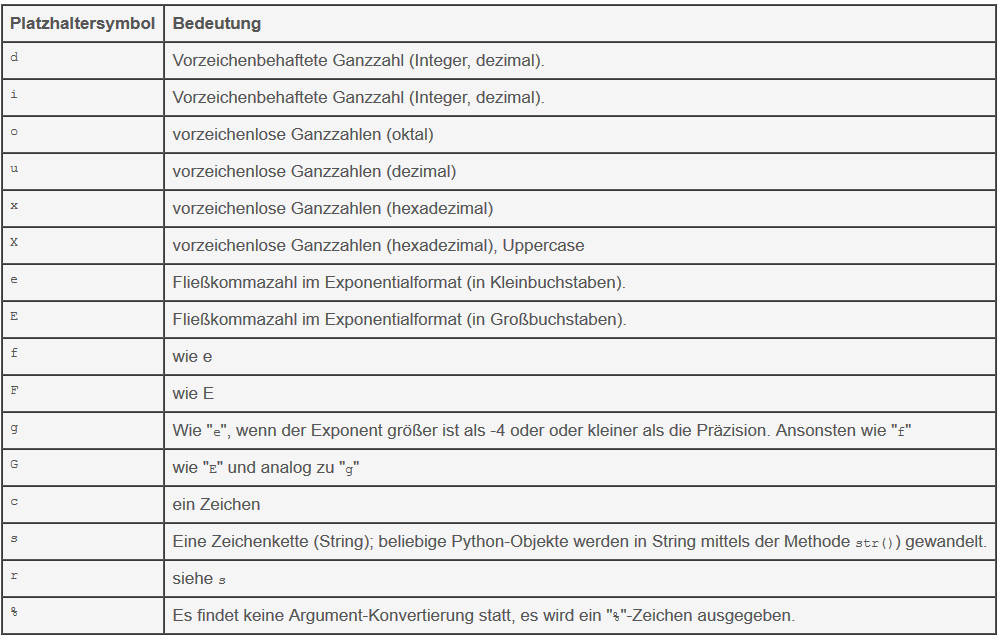
\includegraphics[width=\textwidth]{chapters/inputOutput/FormatierungSymbole.png}
\end{figure}

Was ist jedoch, falls die Ausgabe eine bestimmte L�nge haben soll?
Mit Hilfe der Syntax der Modulo-Arithmetik k�nnen wir dieses Problem l�sen.

 \begin{lstlisting}[language=Python, label=formatInOut:lst:syntax]
 # Modulo-Arithmetik Syntax
 
%[Flag][Minimum der Gesamtl�nge].[Pr�zision][Typ]
 \end{lstlisting}
 
 Das Minium der Gesamtl�nge bringt gro�e Vorteile mit sich, wenn wir z.B. einen linksb�ndigen Text ausgeben wollen. Alle Ausgaben, die k�rzer als das vorgegebene Minimum sind, werden mit Leerzeichen aufgef�llt.
 
 \warning{Es handelt sich hierbei um das Minimum der Gesamtl�nge. Alle Ausgaben die gr��er sind, werden nicht beschr�nkt und in voller L�nge ausgegeben!}
 
 Mittels Punkt k�nnen wir folgend die Pr�zision einstellen, was bei einem \emph{Float}-Datentyp die Nachkommastellen bestimmt. Alle Zahlen werden zu der angegebenen Nachkommastelle aufgerundet!
 
 \begin{lstlisting}[language=Python, label=formatInOut:lst:precision]
 # Modulo-Arithmetik Pr�zision
 
print("Eine Zahl %f" % (1.234))
print("Eine gerundete Zahl %.2f)

# Ausgabe:
# Eine Zahl 1.234
# Eine gerundete Zahl 1.23
\end{lstlisting}
 
\subsection{Formatierung mit format()}

Python bietet uns f�r die Formatierung von String-Elementen die Methode \emph{format()}.

 \begin{lstlisting}[language=Python, label=formatInOut:lst:formatMethod]
# Syntax der format()-Methode 

string.format(par0, par1, ..., key0=val0, key1=val1, ...)
\end{lstlisting}

\emph{format()} ersetzt markierte Stellen im gegebenen String durch angegebene Werte (Parameter in \emph{format()}) und liefert diesen zur�ck.
Die Stellen werden durch geschweifte Klammern markiert und mittels Modulo-Arithmetik pr�zisiert. In der geschweiften Klammer geben wir als erstes den Index (oder das Schl�sselwort) des Parameters an.

 \begin{lstlisting}[language=Python, label=formatInOut:lst:formatString]
# format() mit gegebenem String 

str = "Hallo, {0:s} und {1:s}"
print(str.format("Rainer", "Denis"))
# Ausgabe: 
# Hallo, Rainer und Denis

print(str)
# Ausgabe:
# Hallo, {0:s} und {1:s}

# format() ver�ndert den String nicht,
# sondern liefert den ver�nderten Wert zur�ck

str = str.format("Rainer", "Denis")
print(str)
# Ausgabe: 
# Hallo, Rainer und Denis

# der Wert von 'str' wurde durch den R�ckgabewert
# von format() �berschrieben!

str = "Hallo, {1:s} und {0:s}"
str.format("Rainer", "Denis")
print(str)
# Ausgabe:
# Hallo, Denis und Rainer

# in 'str' wurde der angegebene Index vertauscht

str = "Hallo, {r:s} und {d:s}"
print(str.format(r = "Rainer", d ="Denis"))
# Ausgabe: 
# Hallo, Rainer und Denis

# Angabe von Schl�sselwort-Parametern
\end{lstlisting}

\warning{M�chte man geschweifte Klammern ausgeben, dann werden diese doppelt geschrieben ("'\{\{"' und "'\}\}"')}

Die \emph{format()}-Methode bietet uns au�erdem Ausrichtungsoptionen, was zu besserer Lesbarkeit beitragen kann. Somit k�nnen wir bspw. Werte links- oder rechtsb�ndig ausgeben. Hierf�r gibt man die Formatierungsanweisung an und den Wert des Abstandes bzw. der Gr��e des Platzhalters. Ist das Wort zu kurz, wird der restliche Platz mit Leerzeichen aufgef�llt.

\begin{tabular}{|c | p{8cm}|}
	\hline
	Formatierungsanweisung & Bedeutung \\
	\hline
	< & Text wird linksb�ndig ausgelegt \\
	> & Text wird rechtsb�ndig ausgelegt \\
	\hline
\end{tabular}


\begin{lstlisting}[language=Python, label=formatInOut:lst:formatAlignment]
# Ausrichtung mit Formatierungsanweisung

# linksb�ndig
str = "{0:<10s} {1:d}"
print(str.format("Viereck", 4))
print(str.format("F�nfeck", 5))
print(str.format("Sechseck", 6))

# Ausgabe:
# Viereck    4
# F�nfeck    5
# Sechseck   6


# rechtsb�nding
str = "{0:>10s} {1:d}"
print(str.format("Viereck", 4))
print(str.format("F�nfeck", 5))
print(str.format("Sechseck", 6))

# Ausgabe:
#    Viereck 4
#    F�nfeck 5
#   Sechseck 6
\end{lstlisting}

Python bietet uns f�r \lstinline{Dictionaries} einen einfachen Weg, diese mittels \emph{format()} und der Nutzung von Schl�sselwort-Parametern, auszugeben. 
	
\begin{lstlisting}[language=Python, label=formatInOut:lst:formatDict]
# Formatierung eines Dictionarys

dictMath = {"Dreieck" : "3", 
	   "Viereck" : "4", 
	   "F�nfeck" : "5",

str = "{body}: {corners}"

for geoBody in dictMath
    print(str.format(body=geoBody, 
                     corners=dictMath[geoBody]))
    
# Ausgabe:
# Dreieck: 3
# Viereck: 4
# F�nfeck: 5
\end{lstlisting}


% !TeX root = ../../pythonTutorial.tex
\section{Konsoleneingabe mit input()}
\label{inputInOut}

Mit Hilfe von \lstinline$input()$ erlauben wir dem Nutzer Eingaben �ber die Konsole. Somit erhalten wir den ersten Grad an Interaktion zwischen Nutzer und Programm.

\begin{lstlisting}[language=Python, label=inputInOut:lst:inputDefault]
# die input-Methode

input(prompt)
\end{lstlisting}

Sobald \lstinline$input()$ aufgerufen wird, wartet das Programm mit dem weiteren Ablauf, bis der Nutzer seine Eingabe mit der Eingabetaste best�tigt.
Die \lstinline$input()$-Methode liefert den eingegebenen Wert als String zur�ck.
Damit der Nutzer wei�, was er denn eingeben muss, bietet \lstinline$input()$ den optionalen Standard-Parameter \lstinline$prompt$ an - hierbei handelt es sich um einen leeren String.
Geben wir \lstinline$prompt$ nun einen Wert, wird dieser dem Nutzer f�r die Eingabe angezeigt.

\begin{lstlisting}[language=Python, label=printInOut:lst:inputPrompt]
# die input-Methode mit prompt-Angabe

userName = input("Geben Sie Ihren Namen ein.")
print("Hallo, " + userName)
\end{lstlisting}

\warning{Der Eingabewert des Nutzer liefert immer einen String zur�ck.
Bei gew�nschtem Datentyp, muss \emph{gecasted} werden!}

\kontrollfrage{
	\item[\kontroll] Wie verh�lt sich das Programm bei Aufruf der \lstinline$input()$-Methode?
	\item[\kontroll] Welchen Wert liefert \lstinline$input()$ zur�ck? Um was f�r einen Datentyp handelt es sich?
	\item [\kontroll] Welchen Effekt hat die Angabe des \lstinline{prompt}-Parameters?
}

Bei primitiven Datentypen ist das Umwandeln recht einfach. Bei nicht-primitiven kann es jedoch zu �berraschungen kommen.

\begin{lstlisting}[language=Python, label=printInOut:lst:inputCast]
# die input-Methode mit Typ-Umwandlung

summe = int(input("2 + 3 = "))
print(summe, type(summe), sep=" - ")
# Eingabe: 5
# Ausgabe: 5 - <class 'int'>

geoKoerper = list(input("Geben Sie einige" +
			"geometrische K�rper an"))
print(geoKoerper)
# Eingabe: ["Dreieck", "Viereck"]
# Ausgabe: [' ', '[', '"', 'D', 'r', 'e', 
	'i', 'e', 'c', 'k', '"', ',', 
	' ', '"', 'V', 'i', 'e', 'r', 
	'e', 'c', 'k', '"', ']']
			
print(type(geoKoerper[0]))
# Ausgabe: <class 'str'>

\end{lstlisting}

Python wandelt den String in eine Liste um, jedoch nimmt es jedes einzelne Zeichen der Eingabe als Listenelement. Dies kann durchaus n�tzlich sein, verfehlt hierbei aber das Ziel. Um die geometrischen K�rper als Elemente zu erhalten, nutzen wir die \lstinline$eval()$-Funktion.
\randnotiz{\lstinline$eval()$}
Hierbei wird die Eingabe interpretiert und der entsprechende Datentyp zur�ckgeliefert (Evaluierung).

\tip{eval() funktioniert auch bei anderen Collections!}

\begin{lstlisting}[language=Python, label=printInOut:lst:inputEval]
# die input-Methode mit eval()

geoKoerper = eval(input("Geometrische K�rper: "))
print(geoKoerper)
# Eingabe: ["Dreieck", "Viereck"]
# Ausgabe: ['Dreieck', 'Viereck']
\end{lstlisting}


\kontrollfrage{
	\item[\kontroll] Wie verh�lt sich der R�ckgabewert von \lstinline$input()$, wenn man ihn zu einer Liste umwandelt?
	\item[\kontroll] Welche Methode bietet uns Python an, um den R�ckgabewert wie gew�nscht zu erhalten?
}


% !TeX root = ../../pythonTutorial.tex
\section{Dateien lesen und schreiben}
\label{filehandling:section:dateienlesenundschreiben}

Python bietet nativ M�glichkeiten f�r das Bearbeiten von Dateien. 
Hierf�r werden Objekte erstellt und verwendet, die eine Datei im Quellcode repr�sentieren.
Mithilfe dieser, im folgenden \lstinline$fileObjects$ genannt, l�sst sich der Inhalt einer Datei �ndern und wird gespeichert, 
sobald es im Code mit der \lstinline$close()$-Methode geschlossen wird.

\subsection{Dateitypen}
\label{filehandling:section:filetypes}

In Python werden Dateien in zwei Kategorien eingeteilt. Entweder in Text- oder Bin�rdateien.

Textdateien bestehen aus Zeilen, die aus einer Zeichensequenz bestehen und mit einem \glqq{}End of Line\grqq{}-Zeichen beendet werden. 
Als solches kann beispielsweise ein Zeilenumbruch oder Komma dienen. 

Als Bin�rdateien werden s�mtliche Dateien interpretiert, die keine Textdateien sind. 
Um diese nutzen zu k�nnen, muss der Programmierer eine M�glichkeit zur Verarbeitung bereitstellen. 

In diesem Kapitel werden Beispiele anhand einer Textdatei durchgef�hrt. 

\subsection{Open-Methode}
\label{filehandling:section:open}

Die tragenden Rolle f�r das Bearbeiten von Dateien in Python ist die \lstinline$open()$-Methode. 
Diese erlaubt das Erstellen, �ffnen, Aktualisieren, Lesen und Schreiben einer Datei.

Mithilfe des folgenden Codes wird eine neue Datei erstellt und als \lstinline$fileObject$ ge�ffnet.
\lstinputlisting[language=Python, linerange={1-1,4-5}]{chapters/inputOutput/src/dateienLesenUndSchreiben/FileHandlingReadWrite.py}
\label{filehandling:lst:open}
Zum Erstellen einer neuen Datei wird als erster Parameter ein Dateiname und als zweiter der \lstinline$"x"$-Modus gew�hlt. 
Die Datei wird am gleichen Speicherort, wie die .py-Datei erzeugt, sofern vor dem Dateinamen kein Pfad angegeben wird. 
Sollte an der angegebenen Stelle bereits eine Datei mit dem gew�hlten Namen existieren, bleibt diese unver�ndert und es wird ein Fehler erzeugt. 

Wird das \lstinline$fileObject$ im Code nicht mehr ben�tigt, wird es mit folgender Zeilen-Anweisung geschlossen:
\lstinputlisting[language=Python, linerange={1-1,6-7}]{chapters/inputOutput/src/dateienLesenUndSchreiben/FileHandlingReadWrite.py}
\label{filehandling:lst:close}
Nach einem Schlie�en der Datei wird der verwendete Speicherplatz freigegeben. 
Das Arbeiten ist dann �ber das entsprechende \lstinline$fileObject$ nicht mehr m�glich. 

\tip{Direkt nach Ausf�hren der gew�nschten Operationen, empfiehlt es sich die Datei zu schlie�en. Auf diese Weise wird sichergestellt, dass die Datei nicht unabsichtlich bearbeitet wird.}

F�r die \lstinline$open()$-Methode stehen folgende Modi \randnotiz{Zugriffmodus} zur Verf�gung:

\begin{description}
	\item[x:] Erzeugen einer neuen Datei. 
	Sollte bereits eine Datei mit dem gew�hlten Namen existieren, wird ein Fehler ausgegeben.
	\item[r:] Lesen einer Datei.
	\item[r+:] Lese- und Schreibrechte auf einer Datei.
	\item[a:]  Hinzuf�gen von Inhalt am Ende der Datei. 
	Erzeugt eine neue Datei, falls keine mit dem gew�hlten Namen an der angegebener Pfadangabe existiert.
	\item[a+:] \lstinline$"a"$ wird um das Leserecht auf der Datei erg�nzt.
	\item[w:] Schreiben einer Datei. 
	�berschreibt den Inhalt der Datei. 
	Sollte die Datei mit dem gew�hlten Namen noch nicht existieren, wird eine neue erzeugt.
	\item[w+:] \lstinline$"w"$ wird um das Leserecht auf der Datei erg�nzt.
	\item[t, b:] Angabe, ob die Datei als Text- \lstinline$"t"$ oder Bin�rdatei \lstinline$"b"$ interpretiert werden soll. 
	Diese Modi k�nnen jeweils zu den anderen hinzugef�gt werden. Standardm��ig wird die Datei als Text interpretiert, \lstinline$"t"$ kann hierbei weggelassen werden.
\end{description}

\lstinputlisting[language=Python, firstline=1,lastline=9]{chapters/inputOutput/src/dateienLesenUndSchreiben/FileHandling.py}
\label{filehandling:lst:opentype}


\subsection{Methoden}
\label{filehandling:section:methods}

Die zuvor erstellte Datei hat noch keinen Inhalt. 
Um dies zu �ndern, wird die \lstinline$datei.txt$ im \lstinline$"w"$-Modus ge�ffnet.
Danach kann der Datei �ber die \lstinline$write()$-Methode wie folgt eine Textzeile hinzugef�gt werden.
\lstinputlisting[language=Python, linerange={1-1,9-13}]{chapters/inputOutput/src/dateienLesenUndSchreiben/FileHandlingReadWrite.py}
\label{filehandling:lst:openwrite}
Mithilfe der \lstinline$writelines()$-Methode kann die Datei mit einer List von String-Werten beschrieben werden.
\lstinputlisting[language=Python, linerange={1-1,15-23}]{chapters/inputOutput/src/dateienLesenUndSchreiben/FileHandlingReadWrite.py}
\label{filehandling:lst:openwritelines}
Die Datei in dem Beispiel wurde erstellt, ge�ffnet, beschrieben und �berschrieben. 
Als n�chstes soll der Inhalt aus der Datei auf der Konsole ausgegeben werden. 
Hierzu wird der Modus, in dem die \lstinline$datei.txt$ ge�ffnet wird, auf \lstinline$"r"$ gestellt. 
Die \lstinline$read()$-Methode liefert den Inhalt als String, welcher �ber \lstinline$print()$ ausgegeben wird.
\lstinputlisting[language=Python, linerange={1-1,25-34}]{chapters/inputOutput/src/dateienLesenUndSchreiben/FileHandlingReadWrite.py}
\label{filehandling:lst:openread}
Soll eine einzelne Zeile ausgegeben werden, kann die \lstinline$readline()$-Methode verwendet werden. 
Mittels eines int-Werts als Parameter kann eine Grenze festgelegt werden, die bestimmt, bis zu welcher Position die Zeile ausgelesen werden soll. 
Ohne Angabe eines Parameters wird die gesamte Zeile ausgelesen.
Dies gilt sowohl f�r die \lstinline$read()$- als auch f�r die \lstinline$readline()$-Methode.

Wird der folgende Code ausgef�hrt, f�llt auf, das die \lstinline$datei.txt$ drei 
Zeilen enth�lt und f�r jede Zeile die Anweisung \lstinline$print(fileObject.readline())$ ben�tigt wird, 
um den Inhalt vollst�ndig auszugeben. 
Folglich muss im\\ 
\lstinline$fileObject$ die aktuelle Leseposition gespeichert sein.
\lstinputlisting[language=Python, linerange={1-1,36-49}]{chapters/inputOutput/src/dateienLesenUndSchreiben/FileHandlingReadWrite.py}
\label{filehandling:lst:openreadline}
	
Anstelle der Ausgabe �ber \lstinline$read()$ oder der mehrfachen Verwendung von \lstinline$readline()$, k�nnen wir auch �ber das \lstinline$fileObject$ iterieren. 
In diesem Fall verwenden wir eine for-Schleife.
\lstinputlisting[language=Python, linerange={1-1,51-63}]{chapters/inputOutput/src/dateienLesenUndSchreiben/FileHandlingReadWrite.py}
\label{filehandling:lst:openreadfor}
Eine weitere Alternative ist die \lstinline$readlines()$-Methode, die eine List mit den Zeilen der Datei als Inhalt liefert.
\lstinputlisting[language=Python, linerange={1-1,65-72}]{chapters/inputOutput/src/dateienLesenUndSchreiben/FileHandlingReadWrite.py}
\label{filehandling:lst:openreadlines}
Wird die \lstinline$readlines()$-Methode zweimal hintereinander verwendet, erhalten wir folgende Ausgabe:
\begin{lstlisting}[language=Python]
# Ausgabe:

['Hallo Welt.\n', 'Das ist ein\n', 'Beispieltext']
[]
\end{lstlisting}

Nach dem ersten Aufruf der Methode befindet sich der Zeiger am Ende des \lstinline$fileObject$. 
Somit kann bei dem zweiten Aufruf kein Inhalt mehr ausgelesen werden.
Mithilfe der \lstinline$tell()$-Methode kann die aktuelle Position des Zeigers ausgegeben werden. 
F�gen wir den folgenden Code vor den \lstinline$readlines()$-Methoden ein, kann der Zeiger verfolgt werden.
\lstinputlisting[language=Python, linerange={1-1,74-87}]{chapters/inputOutput/src/dateienLesenUndSchreiben/FileHandlingReadWrite.py}
\label{filehandling:lst:opentell}
Soll die Ausgabe beider Lists identisch sein, muss der Zeiger an den Anfang zur�ckgesetzt werden. 
In Python existiert f�r diesen Zweck die \lstinline$seek()$-Methode. 
Wird der Zeiger direkt nach der ersten Verwendung der\\
\lstinline$readlines()$-Methode auf die Position \lstinline$0$ zur�ckgesetzt, erhalten wir die gew�nschte Ausgabe.
\lstinputlisting[language=Python, linerange={1-1,89-103}]{chapters/inputOutput/src/dateienLesenUndSchreiben/FileHandlingReadWrite.py}
\label{filehandling:lst:openseek}

\subsection{With-Statement}
\label{filehandling:section:withstatement}

Bisher mussten wir in dem Code-Beispiel die \lstinline$open()$-Methode verwenden und darauf achten, 
dass das \lstinline$fileObject$ mit \lstinline$close()$ nach Gebrauch wieder geschlossen wird.

Alternativ kann das \lstinline$with$-Statement genutzt werden. 
So wird die Datei nach Verwendung automatisch geschlossen, ohne die explizite Angabe von\\
\lstinline$close()$. 
Der Code zum Auslesen der datei.txt sieht wie folgt aus:
\lstinputlisting[language=Python, linerange={1-1,105-113}]{chapters/inputOutput/src/dateienLesenUndSchreiben/FileHandlingReadWrite.py}
\label{filehandling:lst:openwithstatement}

\subsection{Attribute}
\label{filehandling:section:attributes}

Jedes \lstinline$fileObject$ besitzt Attribute, die Auskunft �ber das jeweilige Objekt angeben.
\begin{description}
	\item[closed:] Gibt Auskunft dar�ber, ob die Datei geschlossen wurde. Als R�ckgabe erhalten wir einen boolean-Wert.
	\item[mode:] Liefert den Zugriffsmodus auf die Datei als String zur�ck.
	\item[name:] Liefert den Namen der ge�ffneten Datei als String zur�ck.
\end{description}

\lstinputlisting[language=Python, firstline=0,lastline=12]{chapters/inputOutput/src/dateienLesenUndSchreiben/FileHandlingAttributes.py}
\label{filehandling:lst:openattributes}

% !TeX root = ../../pythonTutorial.tex
\section{JSON}
\label{filehandling:section:json}

JavaScript Object Notation (JSON) ist ein Format f�r den Austausch von Daten, das unabh�ngig von der Programmiersprache ist. Aufgrund von Konventionen,
die dieses Format mit Programmiersprachen aus der C-Familie, wie C, C++, Java oder Python teilt, liefert es eine Programmierern bekannte Textstruktur.

In Python 3 ist nativ das json-Package enthalten, das das Arbeiten mit
dem JSON-Format erm�glicht. Mithilfe des folgenden Codes binden wir das Package in das Projekt ein. 
\lstinputlisting[language=Python, linerange={1-1,3-5}]{chapters/inputOutput/src/jsonInPython/JsonInPython.py}
\label{filehandling:lst:importpackage}

Ein gegebener JSON-String wird �ber die \lstinline$loads()$-Methode in ein in Python existierendes, entsprechendes Objekt geparst.
In diesem Fall wird ein Dictionary angelegt.
\randnotiz{JSON zu Python}
\lstinputlisting[language=Python, linerange={1-1,7-19}]{chapters/inputOutput/src/jsonInPython/JsonInPython.py}
\label{filehandling:lst:loads}

F�r das Umwandeln eines Python-Objekts in einen JSON-String verwenden wir die 
\lstinline$dumps()$-Methode.
\randnotiz{Python zu JSON}
\lstinputlisting[language=Python, linerange={1-1,21-35}]{chapters/inputOutput/src/jsonInPython/JsonInPython.py}
\label{filehandling:lst:dumps}

Konvertieren wir Python- zu JSON-Objekte, werden diese im\\
JSON-�quivalent (JavaScript) angelegt.

Wenn wir einen Dictionary mit mehreren Schl�ssel-Objekt-Paaren anlegen,
werden wir bei der Ausgabe des JSON-Objekts feststellen, dass diese auf eine Zeile beschr�nkt sind. 
\lstinputlisting[language=Python, linerange={1-1,37-55}]{chapters/inputOutput/src/jsonInPython/JsonInPython.py}
\label{filehandling:lst:format1}

Zur Formatierung unserer Ausgabe verwenden wir die \lstinline$dumps()$-Methode.
Mithilfe des \lstinline$indent$-Parameters k�nnen wir festlegen, ob und wie weit die Textstruktur einger�ckt werden soll. 
Der \lstinline$separators$-Parameter legt die\\
Trennzeichen fest und mit \lstinline$sort_keys=True$ wird die Ausgabe der Schl�ssel lexikografisch sortiert.
\lstinputlisting[language=Python, linerange={1-1,37-37,56-81}]{chapters/inputOutput/src/jsonInPython/JsonInPython.py}  
\label{filehandling:lst:format2}




% !TeX root = ../../pythonTutorial.tex
\section{Zusammenfassung}
\label{filehandling:subsection:zusammenfassungdateienlesenundschreiben}

In diesem Kapitel haben wir uns mit dem lesen und beschreiben einer Datei auseinandergesetzt.
Dies geschieht in Python mithilfe eines \lstinline$fileObject$ um eine Datei zu erstellen, �ndern, l�schen und abzuspeichern.
Dabei kann eine Datei als Textdatei oder Bin�rdatei interpretiert werden. 
Eine der wichtigsten Methoden stellt hierbei die \lstinline$open()$-Methode dar. 
Diese erm�glicht uns das Erstellen, �ffnen, Aktualisieren, Lesen und Beschreiben einer Datei.
Dabei ist zu beachten, dass die Datei direkt nach der Ausf�hrung der gew�nschten Operationen mithilfe der \lstinline$close()$-Methode geschlossen wird.
Um dies nicht zu vergessen, besteht in Python auch die M�glichkeit ein automatisches Schlie�en mit dem \lstinline$With$-Statement zu erwirken. 
Abschlie�end haben wir noch den Zugriff auf die wichtigsten Attribute, die ein \lstinline$fileObject$ besitzt, kennengelernt und uns mit dem Standardisierten Datenaustausch mittels JSON besch�ftigt.

% !TeX root = ../../pythonTutorial.tex
\uebung

\aufgabe{inputOutput/01_printBody}
\aufgabe{inputOutput/02_inputList}
\aufgabe{inputOutput/03_minLength}
\aufgabe{inputOutput/04_inputDict}


